\chapter{Theorie}


%%%%%%%%%%%%%%%%%%%%%%%%%%%%%%%%%%%%%%%%%%%%%%%
\section{Charakteristische Gleichung des Standardregelkreises}


Die Übertragungsfunktion des geschlossenen Regelkreises lautet:

\begin{equation*}
	Y(z) = \frac{D(z)\cdot H_0G(z)}{1+K\cdot D(z)\cdot H_0G(z)}
\end{equation*}

Bei der charakteristischen Gleichung werden nur die Polstellen betrachtet, sie lautet also: 

\begin{equation*}
	1+K\cdot D(z)\cdot H_0G(z) = 0
\end{equation*}

%%%%%%%%%%%%%%%%%%%%%%%%%%%%%%%%%%%%%%%%%%%%%%%
\section{Vorgehen beim WOK - Verfahren}

Das Wurzelortskurvenverfahren ist eine Methode zur Analyse, wie sich die Pole eines geschlossenen Regelkreises ändern, wenn der Verstärkungsfaktor K variiert. Das Verfahren läuft wie folgt ab:

\begin{enumerate}
	\item Bestimmen der offenen Übertragungsfunktion $H_0G(z)$
	\item Aufstellen der charakteristischen Gleichung
	\item Identifizieren der Pole und Nullstellen der offenen Übertragungsfunktion
	\item Zeichnen der Wurzelortskurve, beginnend bei den Polen für K=0 und endend an den Nullstellen für K→$\infty$
	\item Überprüfung der Stabilität durch Beobachtung der Lage der Pole innerhalb/außerhalb des Einheitskreises
\end{enumerate}
\newpage

%%%%%%%%%%%%%%%%%%%%%%%%%%%%%%%%%%%%%%%%%%%%%%%
\section{Polstellen bei K = 0}

Für K = 0 erhält man:
\begin{equation*}
	1+0\cdot D(z)\cdot H_0G(z) = 0
\end{equation*}

Somit liegen die Polstellen des geschlossenen Regelkreises mit den Polstellen des offenen Regelkreises überein.

\section{Polstellen für K→ $\infty$}

Für K→$\infty$ dominiert der Term $K\cdot H_0G(z)$ der charakteristischen Gleichung: 
\begin{equation*}
	1+K\cdot D(z)\cdot H_0G(z) = 0 \Longrightarrow K\cdot H_0G(z) = -1
\end{equation*}

Für sehr große Werte von K nähert sich die Gleichung asymptotisch den Nullstellen von $H_0G(z)$, da der Ausdruck nur dann erfüllt ist, wenn $H_0G(z)$ selbst gegen $-\frac{1}{K}$ konvergiert, was wiederum Nullstellenbedingung entspricht.

Die Wurzelortskurven enden also bei K→$\infty$ an den Nullstellen von $H_0G(z)$.


%%%%%%%%%%%%%%%%%%%%%%%%%%%%%%%%%%%%%%%%%%%%%%%%%%%%%%%%%%%%%
\chapter{Aufgaben}

\section*{A 3.1}
Das MATLAB Übertragungssystem mit der gegebenen Streckenübertragungsfunktion kann wie folgt erstellt werden:
\begin{center}
	sys\_cont = tf(1, [0.5, 1.5 , 1]);
\end{center}

\section*{A 3.2}
Ein digitales Übertragungssystem kann direkt eingegeben werden, indem man bei der tf()-Funktion noch eine Abtastzeit mit angibt: 
\begin{center}
	h0g = tf([0.1548, 0.0939], [1, -0.9744, 0.2231], T);
\end{center}

\section*{A 3.3}

Um die kontinuierliche Übertragungsfunktion $G_S(s)$ per Hand in die z-Übertragungsfunktion zu transformieren wird der Laplace-Operator s durch eine diskrete Näherung wie beispielsweise beim Euler-Vorwärts- Euler-Rückwärts- oder Tustin-Verfahren ersetzt. Anschließend wird das Ergebnis so weit umgeformt, dass man einen Bruch aus zwei rationalen Funktionen erhält.

\newpage

\section*{A 3.4}

Der Matlab Befehl für diese Transformation lautet wie folgt:
\begin{center}
	sys\_disc = c2d(sys\_cont, T, 'zoh');
\end{center}

Man erhält damit die gleiche Übertragungsfunktion wie angegeben.


\section*{A 3.5}
Folgende Verfahren können mit der c2d Funktion zur Transformation genutzt werden:

\begin{enumerate}
	\item \textbf{'zoh':} Zero-order Hold
	\item \textbf{'foh':} Triangle approximation
	\item \textbf{'impulse':} Impulse invariant discretization
	\item \textbf{'tustin':} Bilinear method
	\item \textbf{'matched':} Zero-pole matching method
	\item \textbf{'least-squares':} Least-squares method
	\item \textbf{'damped':} Damped Tustin approximation
\end{enumerate}

\section*{A 3.6}
Folgende Befehle führen die bilineare Transformation durch:
\begin{center}
	PI\_cont = tf([K, K], [1, 0]);\\
	PI\_disc = c2d(PI\_cont, T, 'tustin');
\end{center}

\newpage

\section*{A 3.7}

Die charakteristische Gleichung für den digitalen Regelkreis mit PI-Regler lautet:

\begin{equation*}
	1 + K\cdot \frac{1,25z - 0,75}{z - 1}\cdot \frac{0,1548z + 0,0939}{z^2 - 0,9744z + 0,2231}
\end{equation*}


\section*{A 3.8}

Nullstellen:
\begin{itemize}
	\item $x_1 = -0,6065$
	\item $x_2 = 0,6$
\end{itemize}
Polstellen:
\begin{itemize}
	\item $p_1 = 1$
	\item $p_2 = 0,6065$
	\item $p_3 = 0,3679$
\end{itemize}
\newpage


\section*{A 3.9}

Abbildung \ref{wok} zeigt die Wurzelortskurve des Systems. Sie beginnt in den Polstellen des offenen Regelkreises und endet in den Nullstellen des offenen
Regelkreises.

\begin{figure}[h]
	\centering
	\includegraphics[width=1\linewidth]{images/wok.png}
	\caption{Wurzelortskurve}
	\label{wok}
\end{figure}


\section*{A 3.10}

Da der Punkt auf der WOK für K=4 wesentlich näher am Einheitskreis liegt, als der Punkt für K = 0.9, ist zu erwarten, dass das System mit geringerer Verstärkung eine deutlich kleinere Überschwingweite und Ausregelzeit als das System mit der höheren Verstärkung hat. Abbildung \ref{sa} bestätigt diese Vermutung.
\newpage

\section*{A 3.11}

\begin{figure}[h]
	\centering
	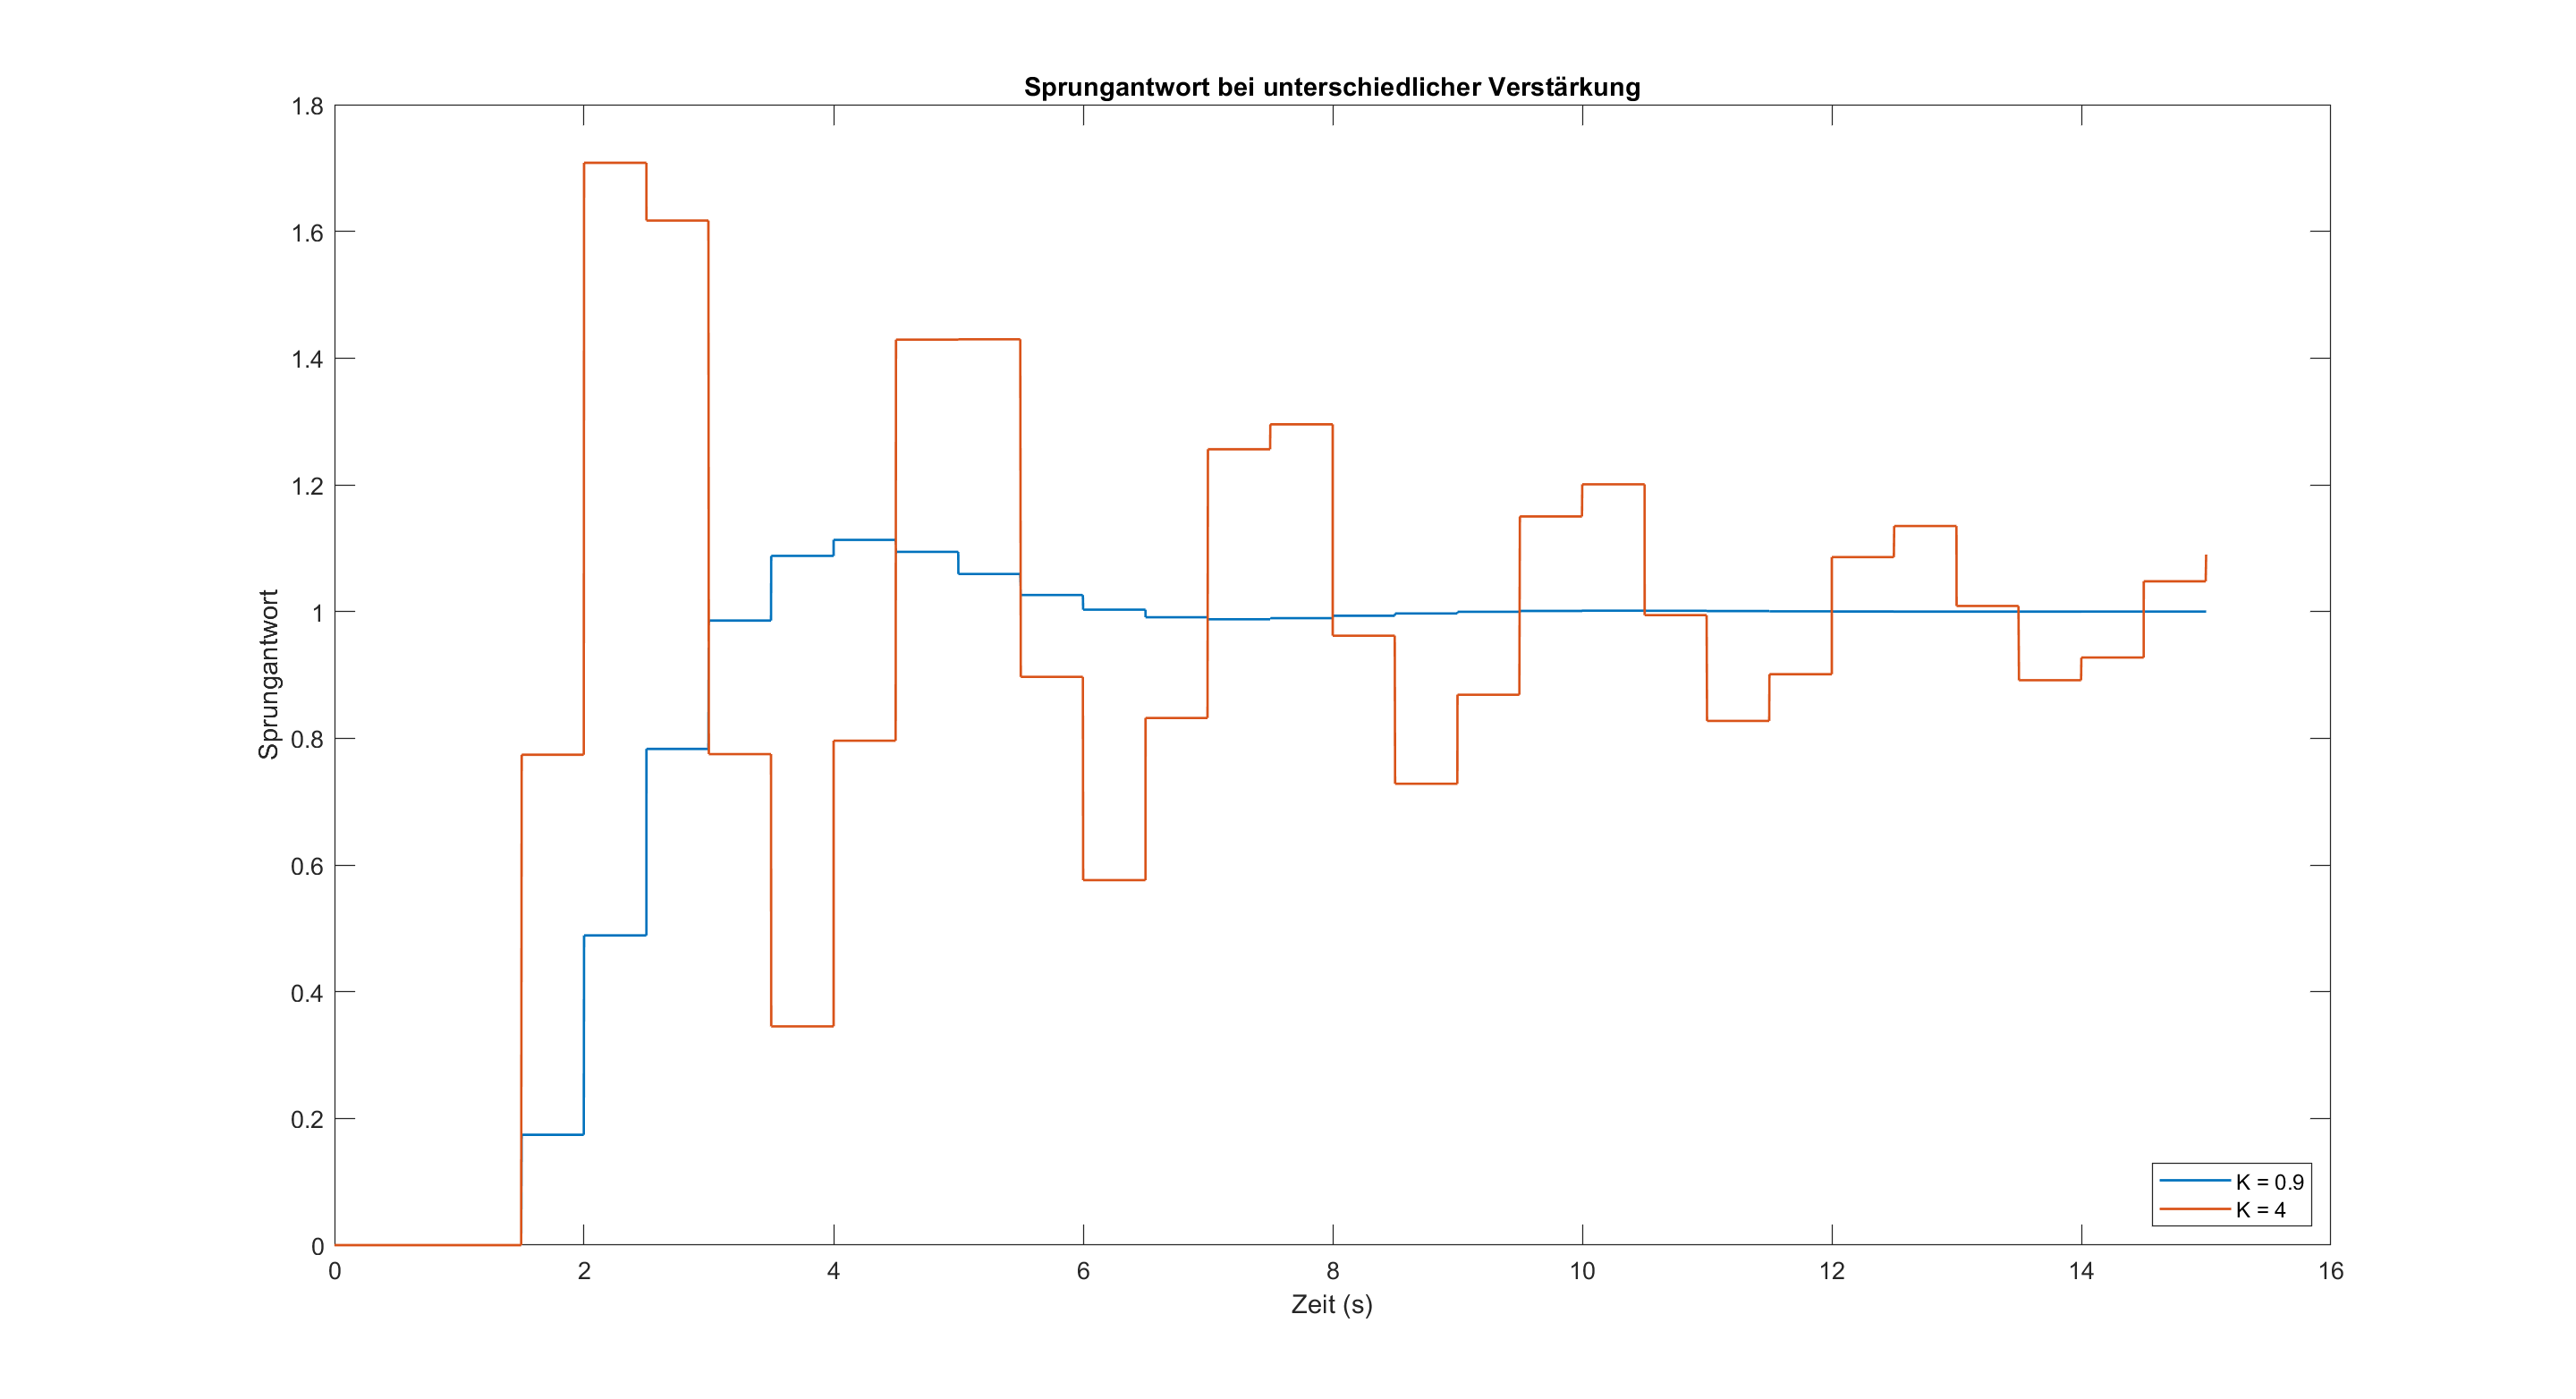
\includegraphics[width=1\linewidth]{images/sprungantworten.png}
	\caption{Sprungantworten bei verschiedenen Reglerverstärkungen}
	\label{sa}
\end{figure}





























